\section{Подключение робота к сети}
\subsection{Общие замечания}
Подключение Robotino к сети обеспечивается маршрутизатором TL-WR702N, находящимся внутри командного блока (см.~рис.~\ref{img_robotino_router}а).
Для <<общения>> с роботом через сеть его можно настроить на работу в одном из двух режимах: точки доступа и клиента.

\begin{figure}[h]
	\begin{minipage}[h]{0.49\linewidth}
		\centering{ 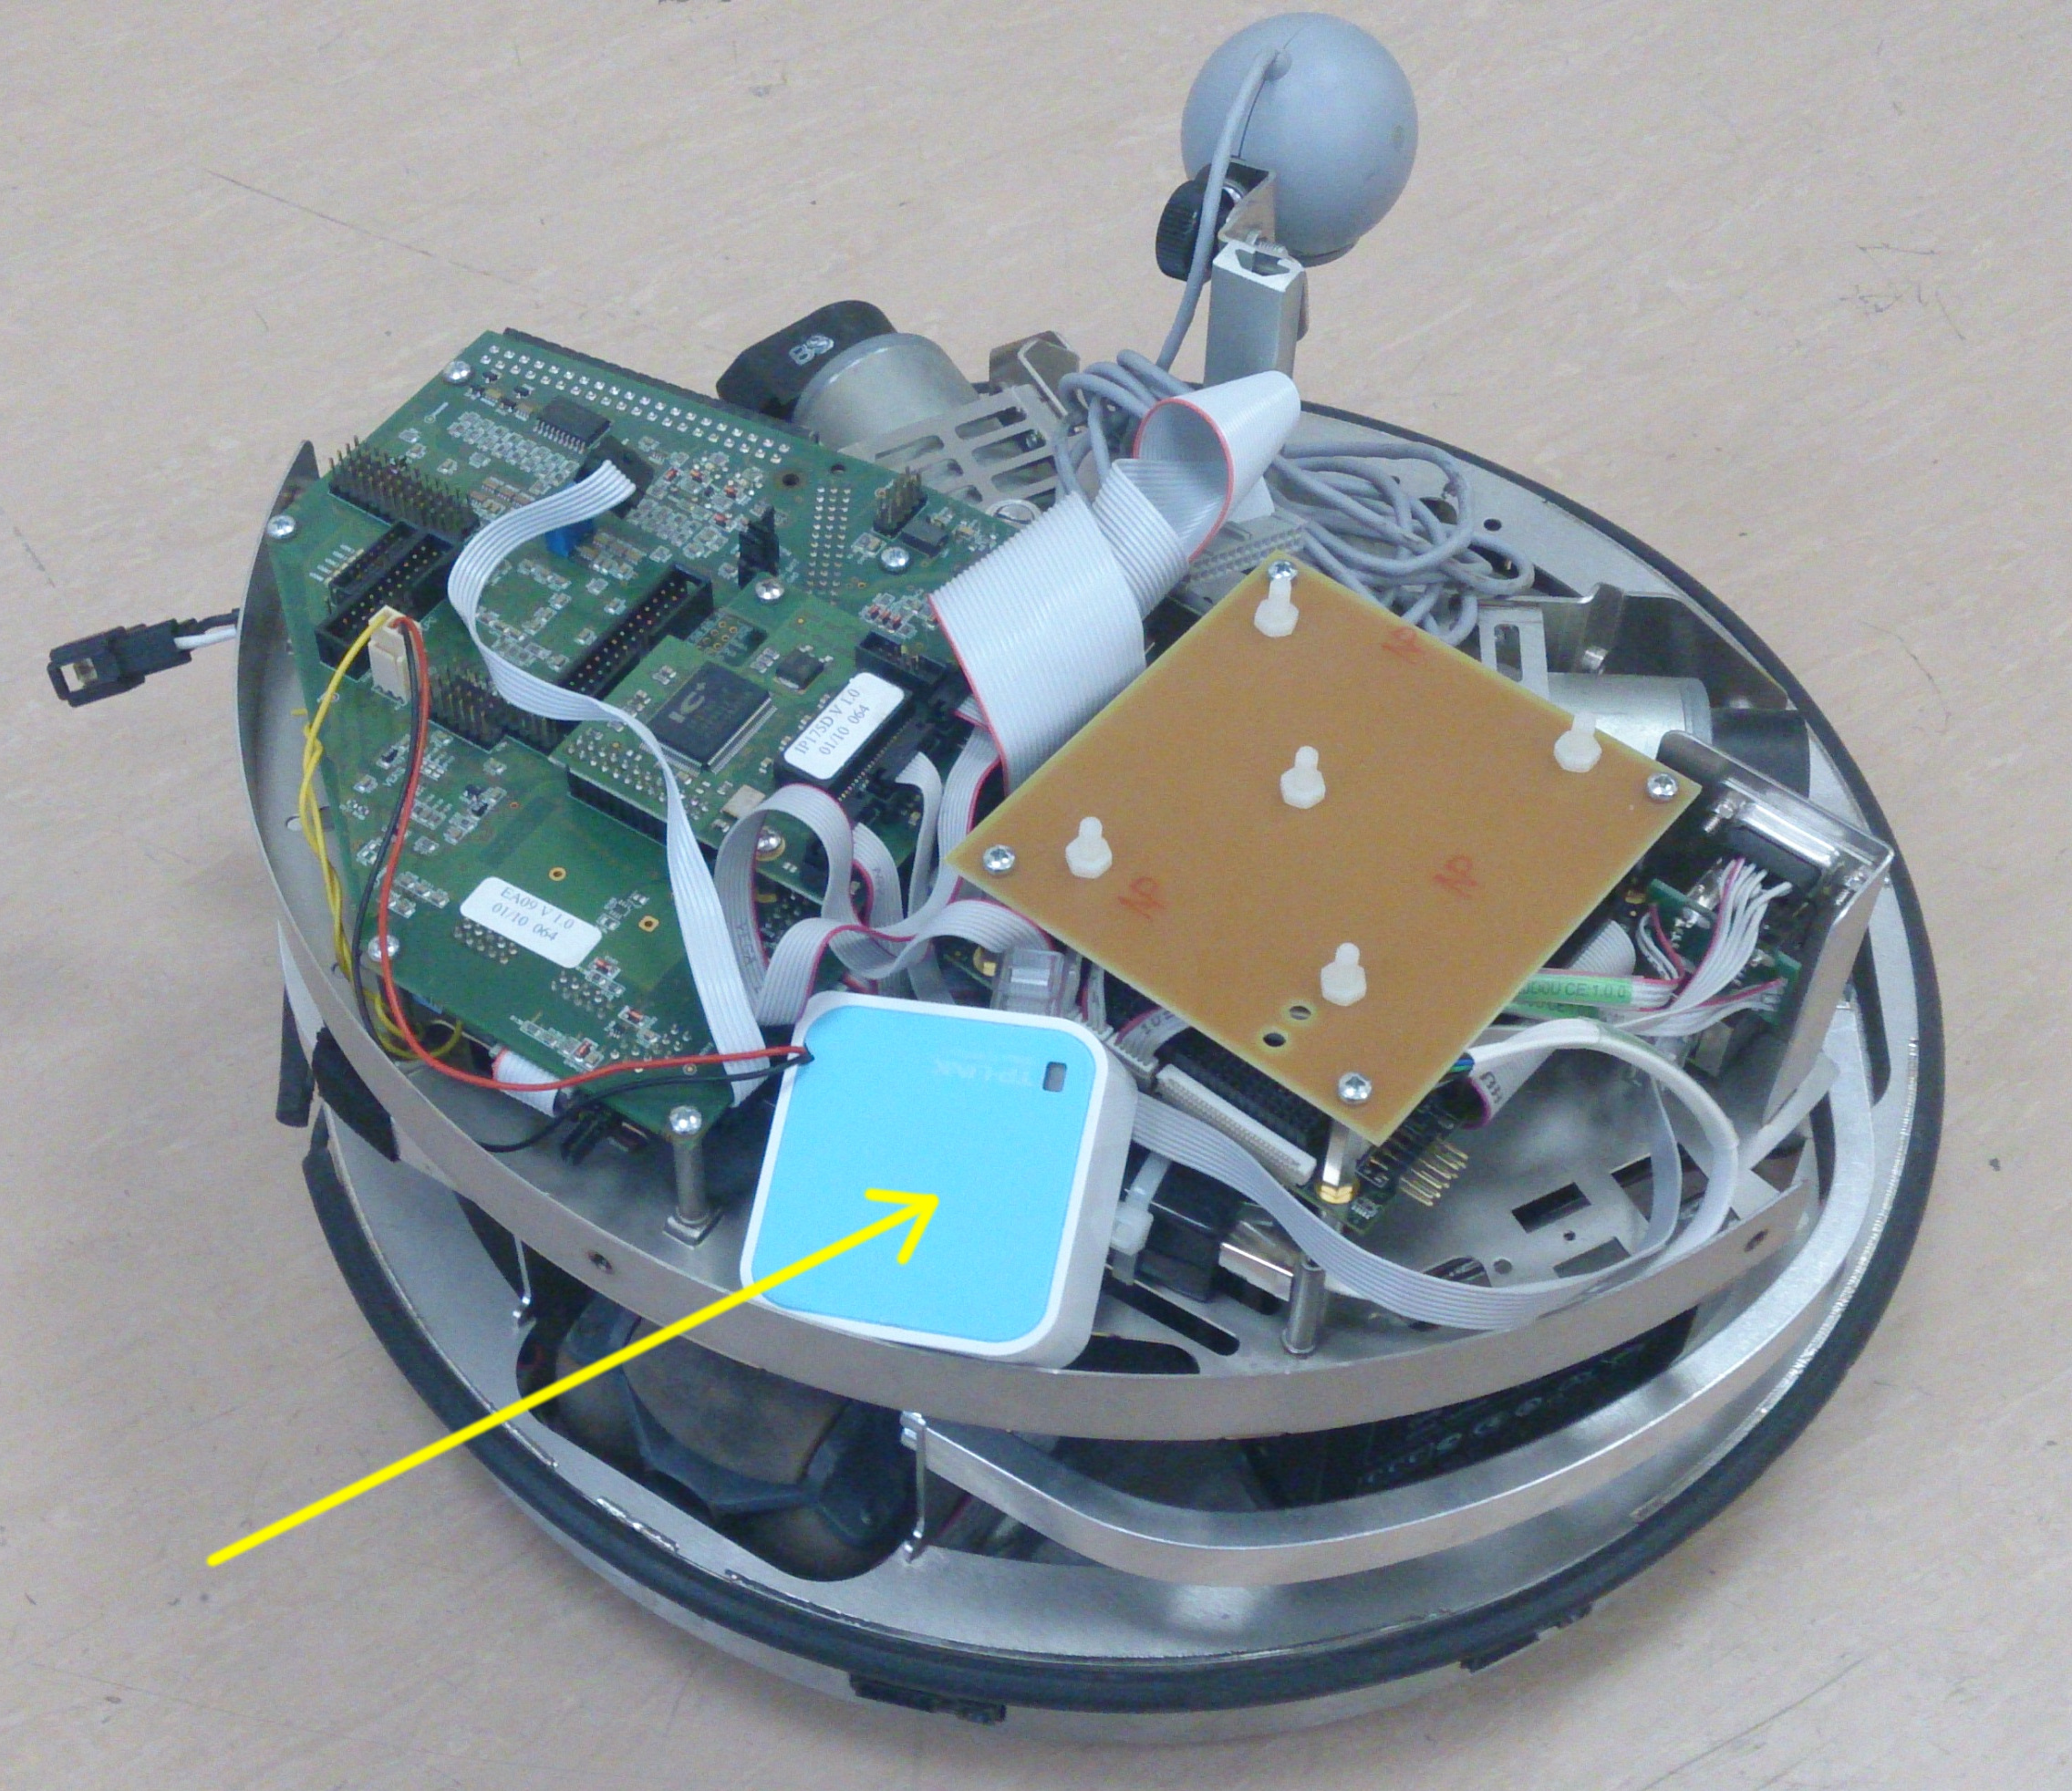
\includegraphics[height = 5.3cm]{router_inside.JPG} \\ a)}
	\end{minipage}
	\hfill
	\begin{minipage}[h]{0.49\linewidth}
		\centering{ 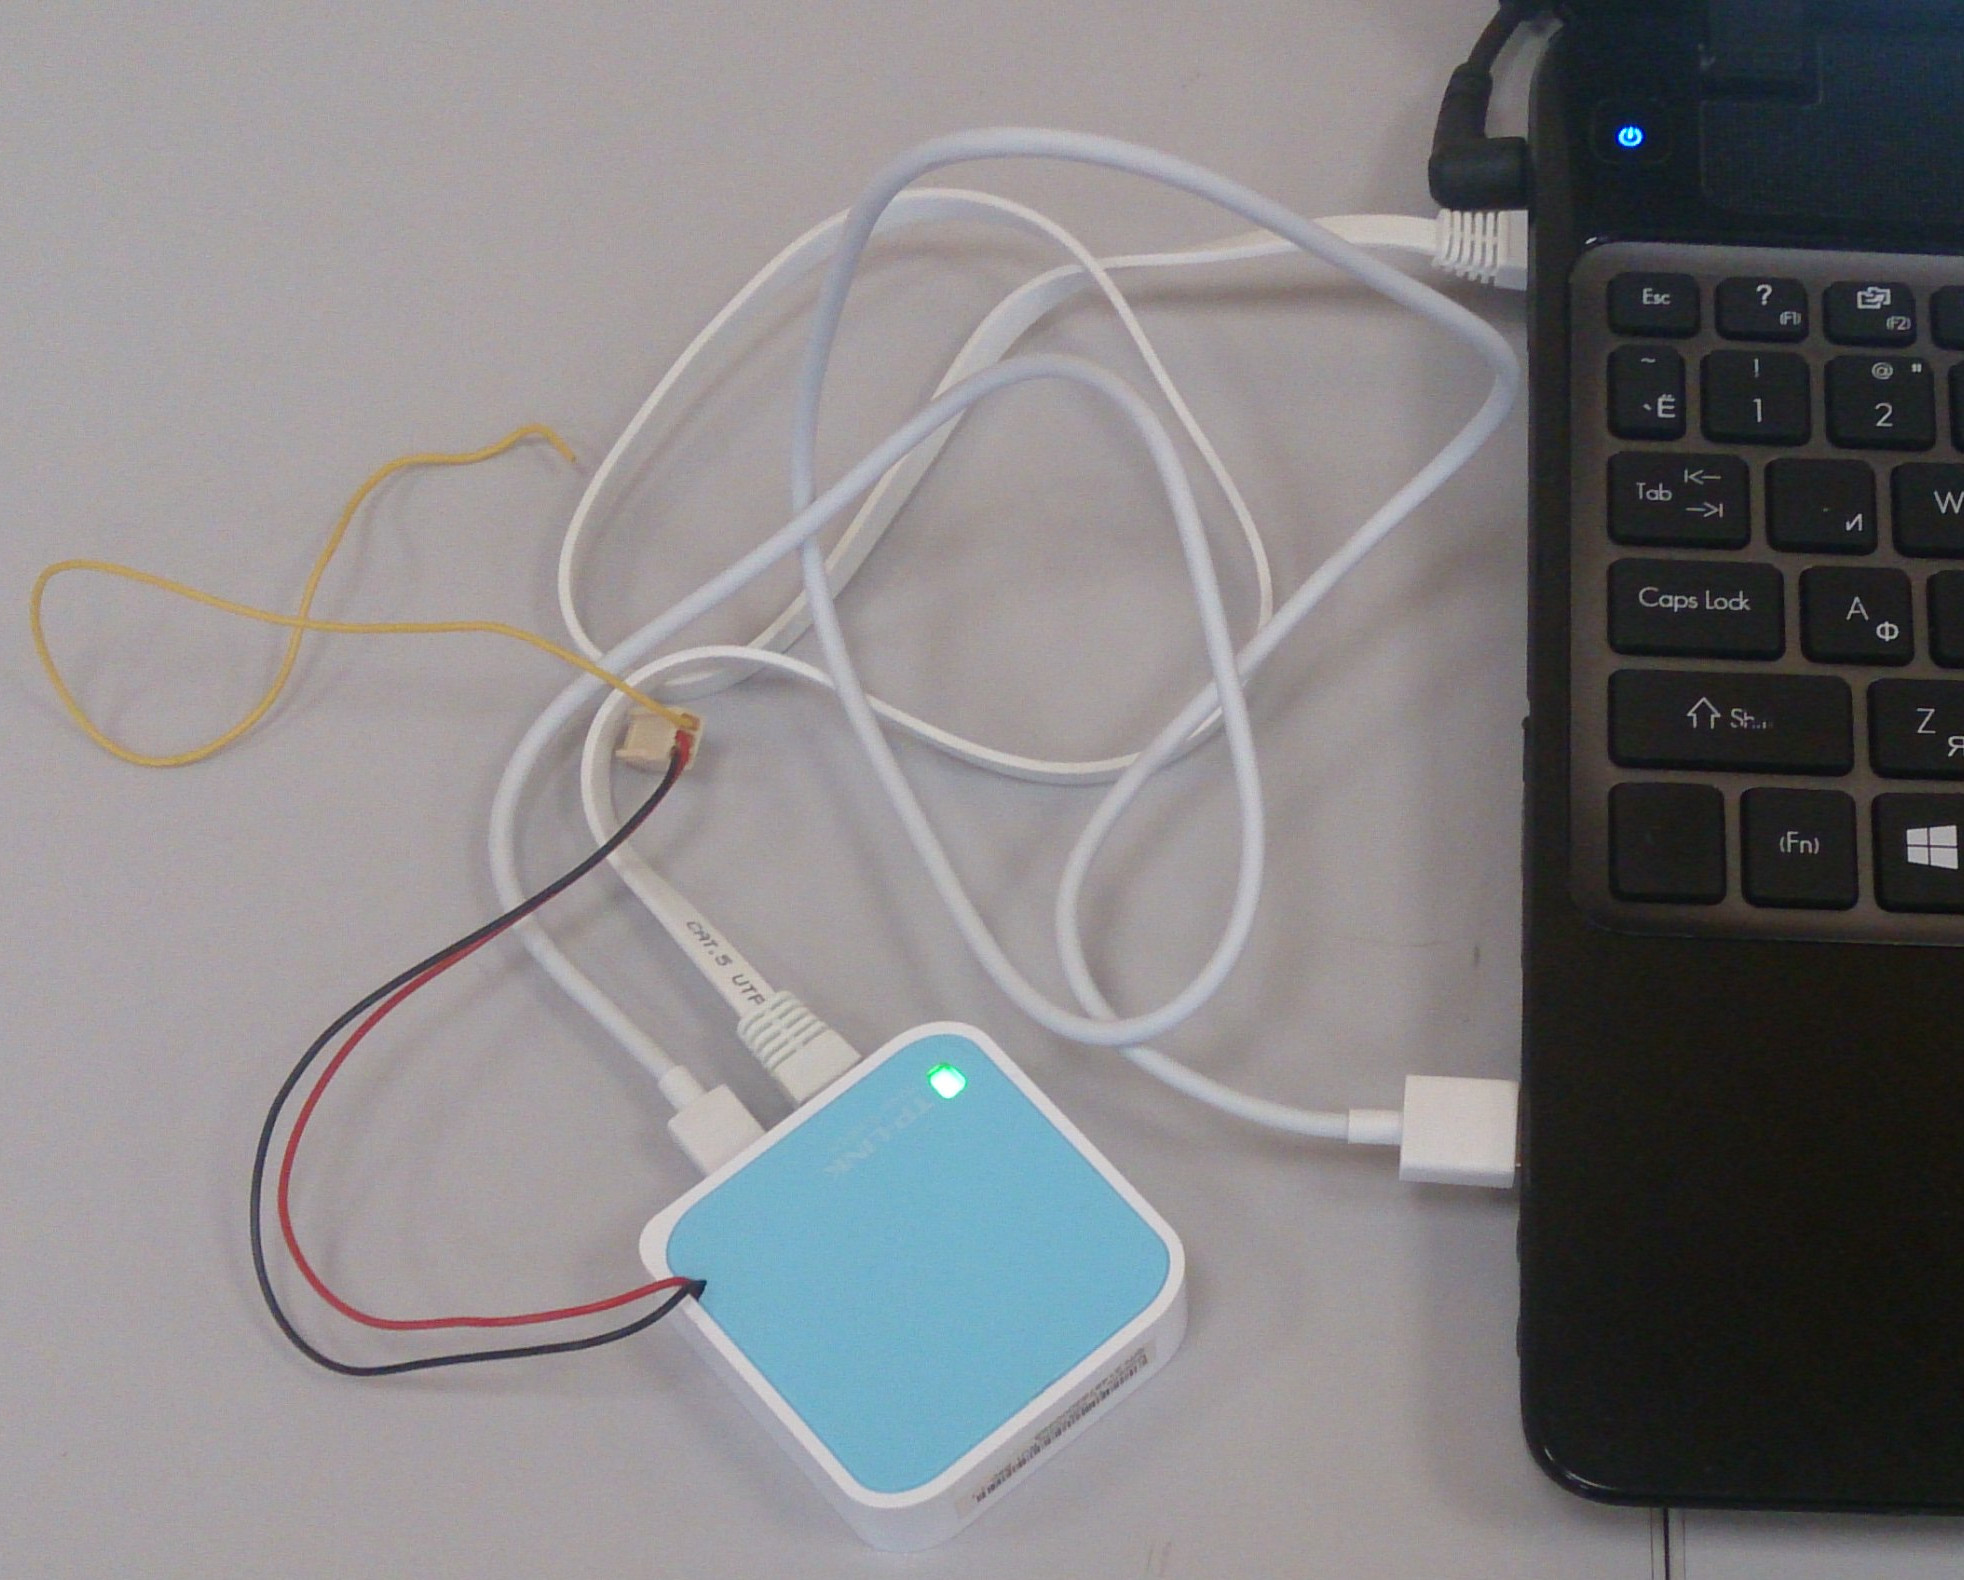
\includegraphics[height = 5.3cm]{router_to_pc.JPG} \\ б)}
	\end{minipage}
	\caption{Маршрутизатор TL-WR702N: a~--- внутри командного блока робота, б~--- подключенный~к~ПК.}
	\label{img_robotino_router}
\end{figure}

Для настройки роутера в первую очередь необходимо к нему подключиться.
Сделать это можно двумя способами~--- см.~п.~\ref{part_with_removing} и \ref{part_without_removing}.



\subsection{Подключение роутера с его предварительным извлечением}\label{part_with_removing}
Извлеките из выключенного робота его CF~карту, предварительно нажав на специально предназначенную для этого кнопку (обведена желтым контуром на рис.~\ref{img_remove_cover}).
Отверните 4~показанные на рис.~\ref{img_remove_cover} красными стрелками винта и снимите крышку командного блока.
Далее отсоедините роутер от присоединенных к нему кабелей питания и Ethernet.
Извлеченный роутер подключите к своему компьютеру с помощью mini-USB и Ethernet кабелей (см.~рис.~\ref{img_robotino_router}б).
Далее нажмите и держите кнопку сброса на роутере до тех пор, пока не замигает его индикаторный светодиод.
Подождите пока роутер не перезагрузится примерно минуту.
Далее откройте на своем компьютере <<Сетевые соединения>> и подключитесь к проводному соединению, созданному роутером (этот процесс может пройти автоматически).
Откройте браузер и введите в его адресной строке IP-адрес роутера (после перезагрузки устройства он сбрасывается до 192.168.0.254).
Далее в открывшемся окне введите логин: admin и пароль: admin.
Роутер готов к настройке.




\subsection{Подключение роутера без его предварительного извлечения}\label{part_without_removing}
Подключите свой компьютер к роботу с помощью Ethernet кабеля, используя тот Ethernet порт робота, который обозначен с помощью~2 на рис.~\ref{img_gen_view_of_robotino}.
Далее откройте на своем компьютере <<Сетевые соединения>> и подключитесь к проводному соединению, созданному при указанном подключении (этот процесс может пройти автоматически).
Там же (в <<Сведения о соединении>>) или иным образом\footnote{Например, с помощью команды ifconfig в *nix системах.} узнайте IP, который получил ваш компьютер в этом соединении.
Просканируйте данную сеть, например, с помощью утилиты nmap, передав ей в качестве аргумента этот IP (команду целиком можно видеть на рис.~\ref{img_nmap}).
Откройте браузер и введите в его адресной строке IP-адрес маршрутизатора, определенный с помощью nmap.
Далее в открывшемся окне введите логин: admin и пароль: admin.
Роутер готов к настройке.

\begin{figure}[h]
	\centering{ 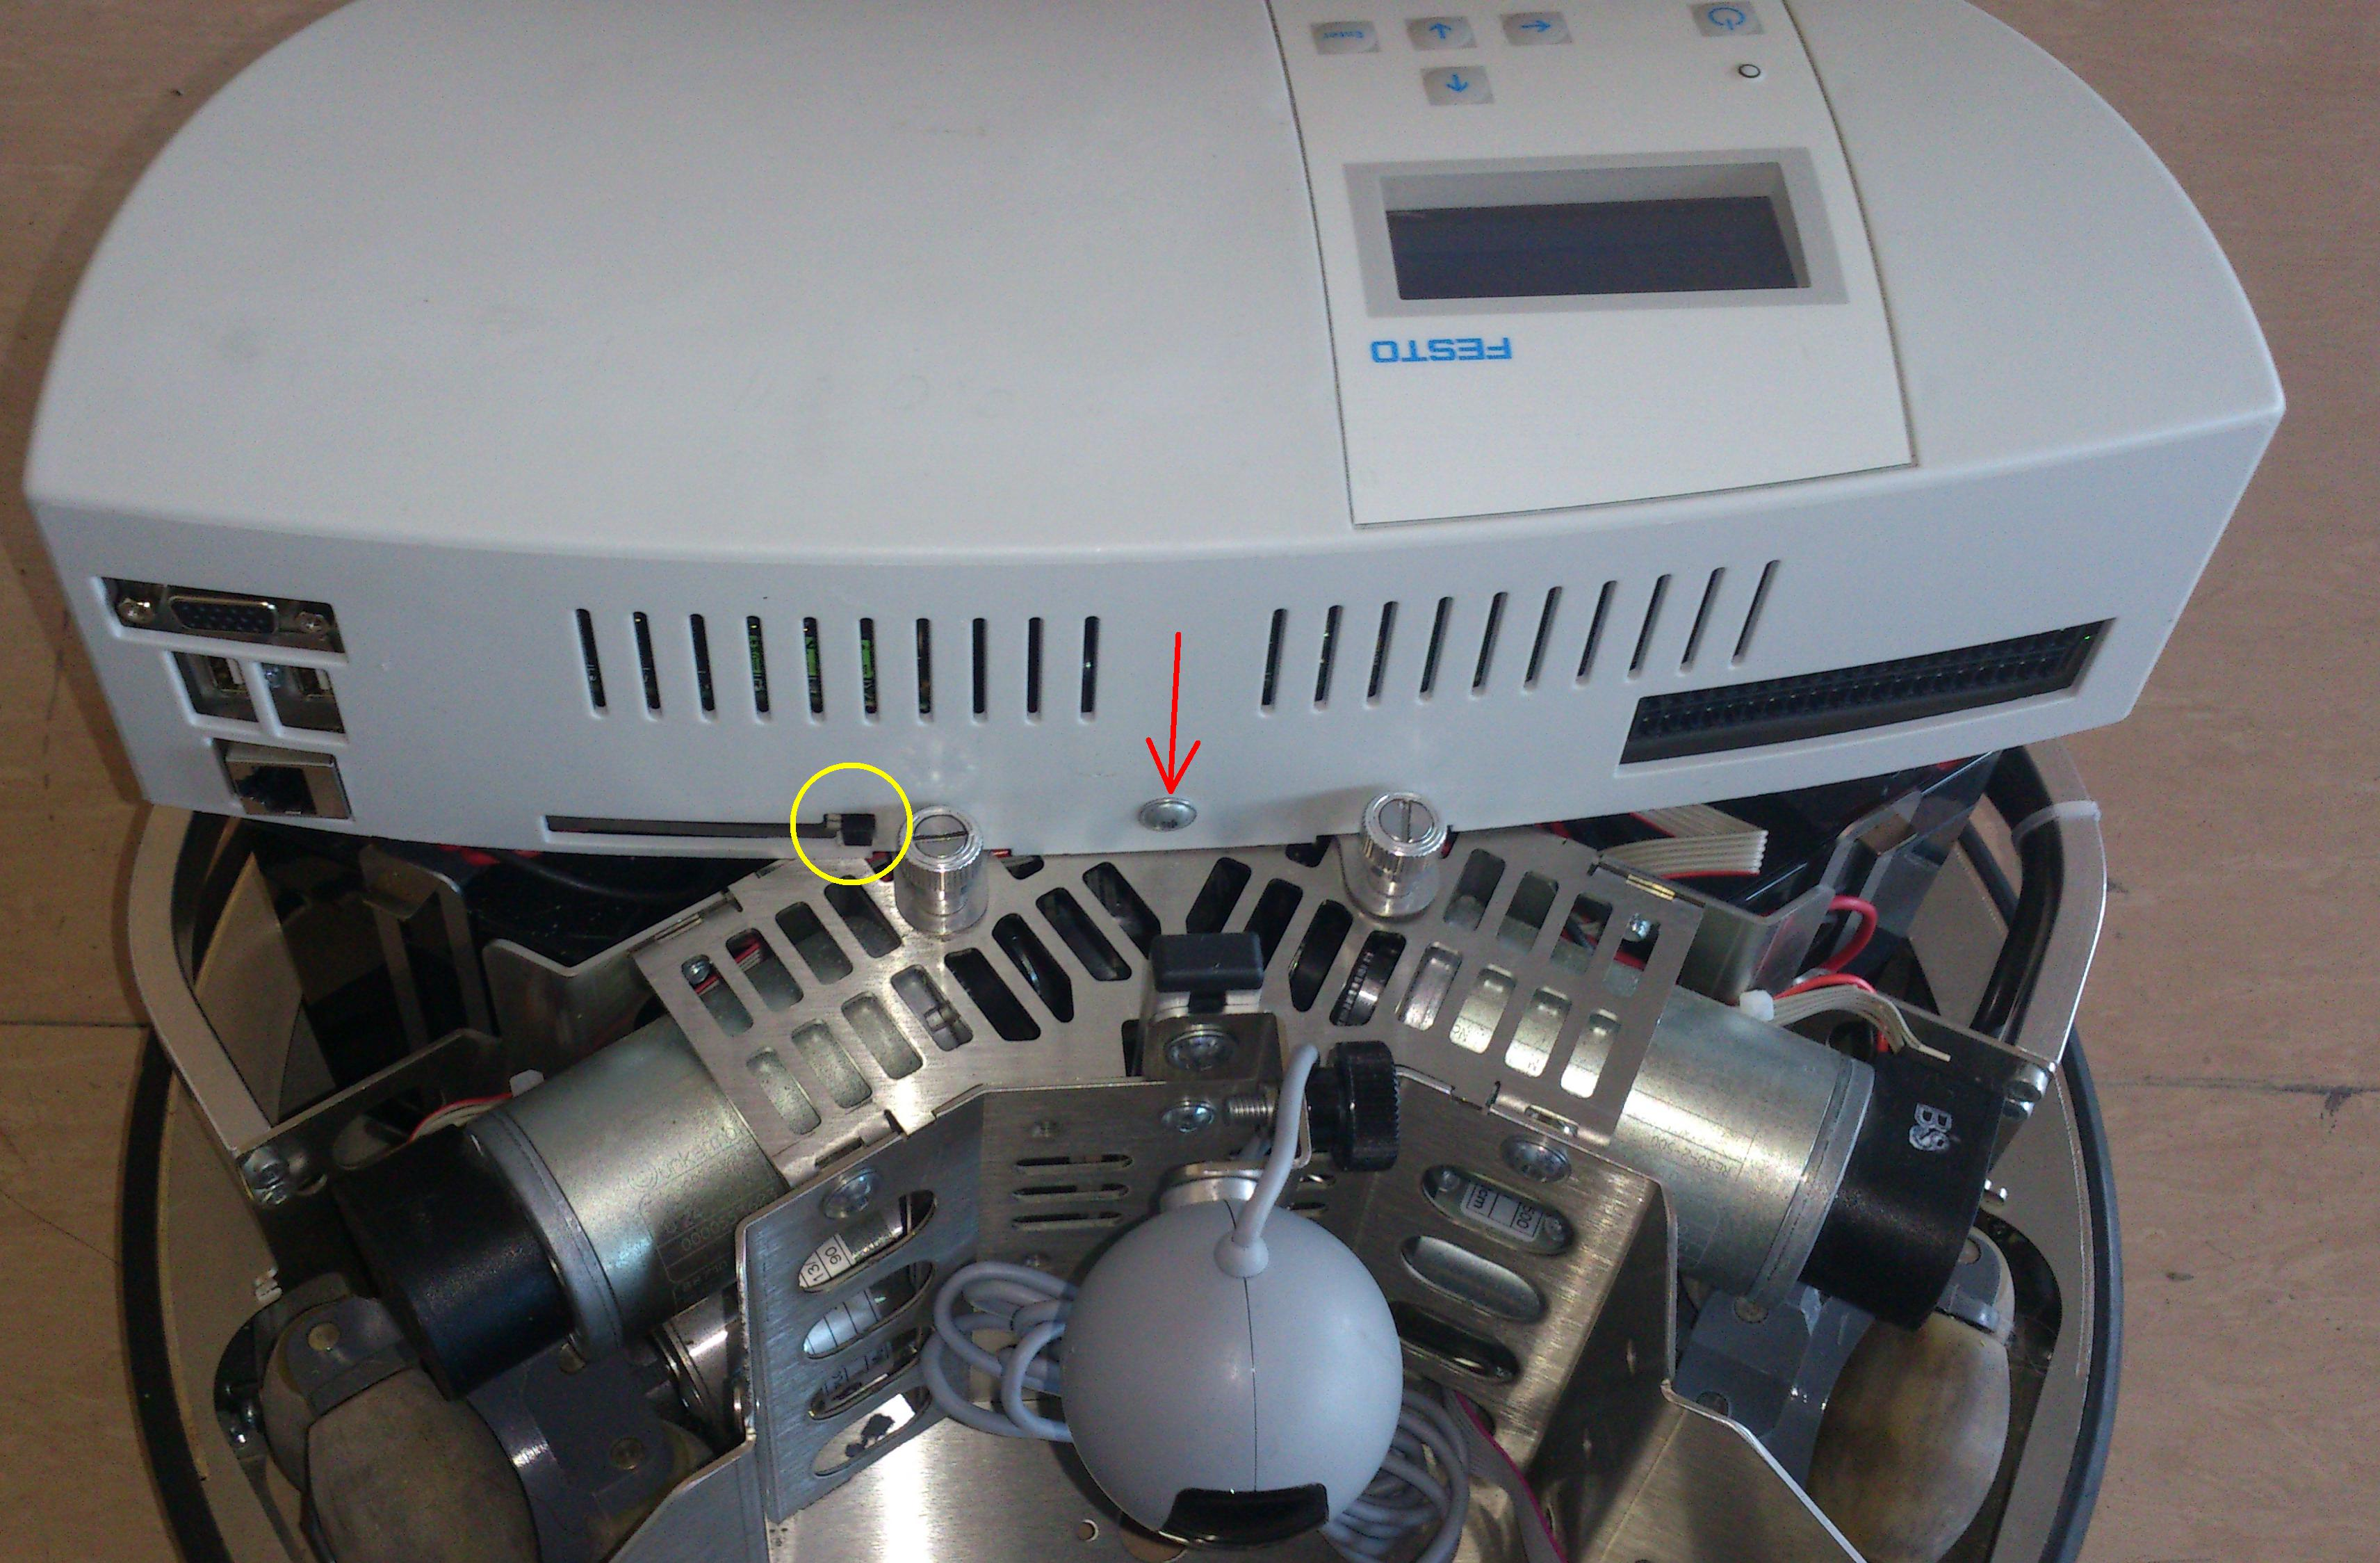
\includegraphics[height = 5.9cm]{remove_cover_1.jpg} }
	\hfill
	\centering{ 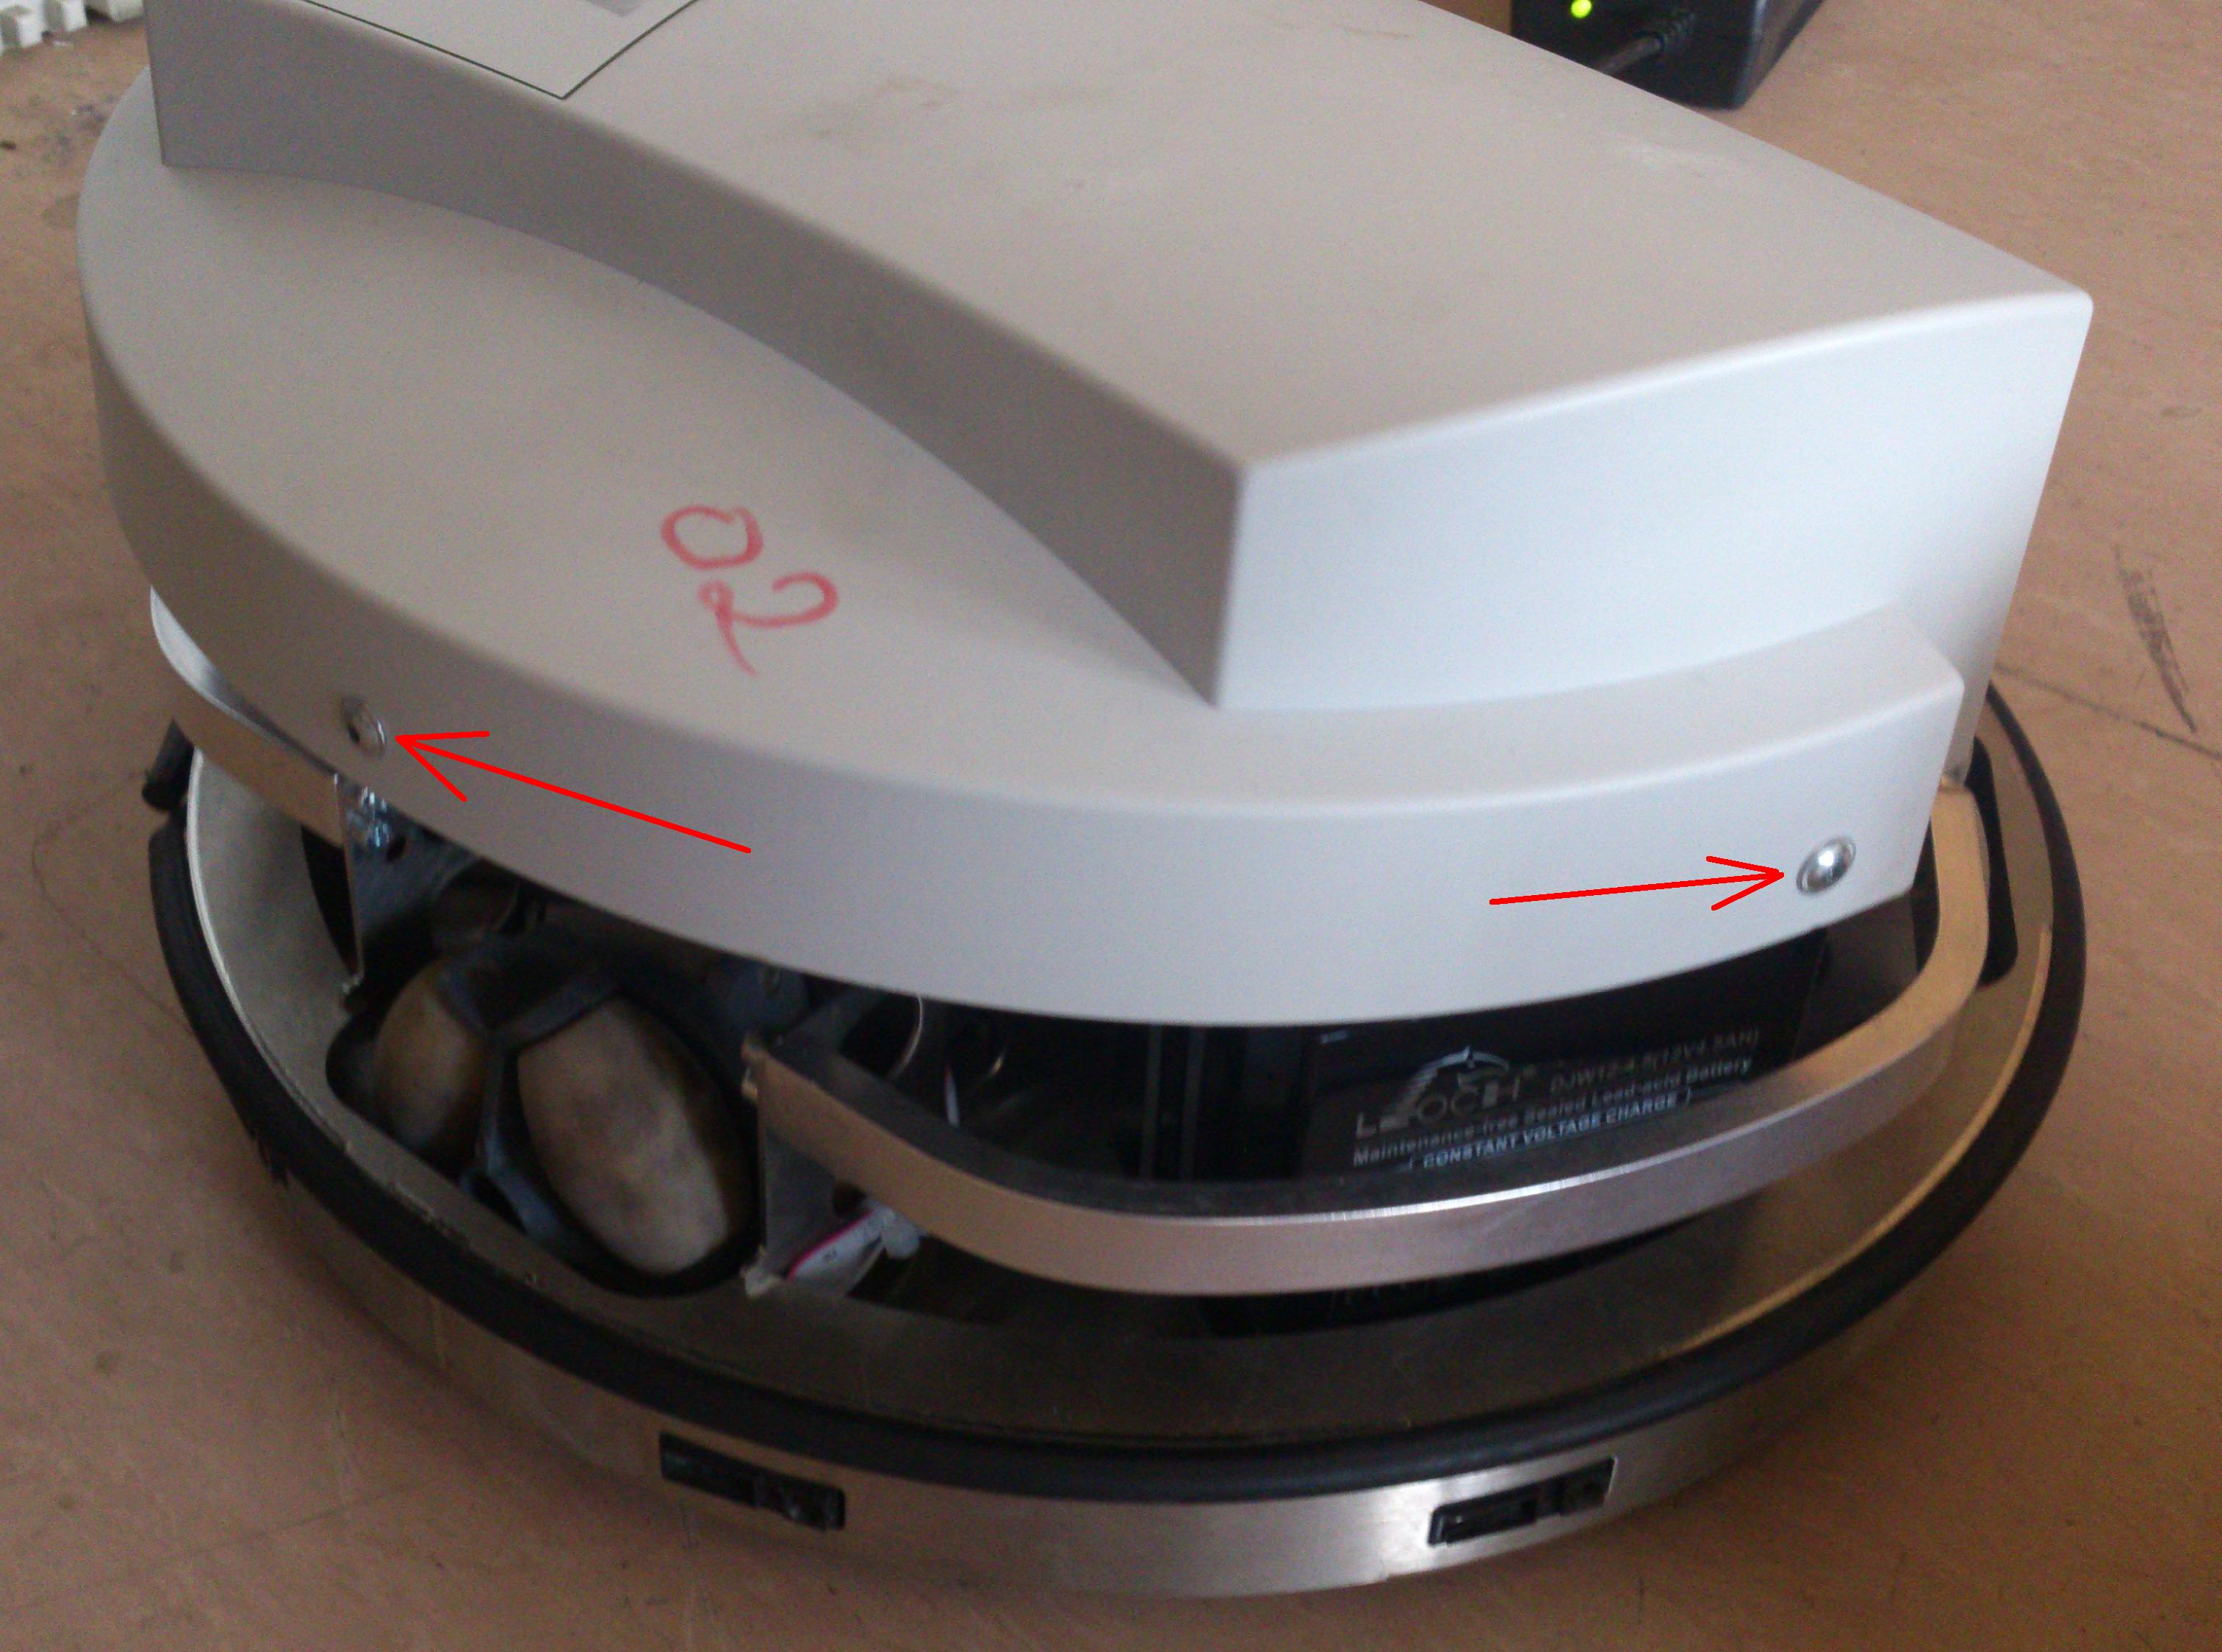
\includegraphics[height = 5.9cm]{remove_cover_2.jpg} }
	\caption{Винты, фиксирующие крышку командного блока робота.}
	\label{img_remove_cover}
\end{figure}




\subsection{Настройка роутера на работу в режиме точки доступа}
\begin{quote}
\textbf{Минусы}: При работе маршрутизатора в этом режиме с одного компьютера можно «общаться» только с одним роботом.\\
\textbf{Плюсы}: Рабочая сеть всегда с собой (с роботом).
\end{quote}

Для настройки работы роутера в режиме точки доступа откройте вкладку <<Быстрая настройка>> (см.~рис.~\ref{img_net_settings}).
Выполните все требуемые действия, выбрав при этом пункт <<Точка доступа>> в качестве желаемого режима работы роутера.



\subsection{Настройка роутера на работу в режиме клиента}
\begin{quote}
\textbf{Плюсы}: При работе маршрутизатора в этом режиме с одного компьютера можно «общаться» с любым количеством роботов.\\
\textbf{Минусы}: Нужна внешняя Wi-Fi сеть.
\end{quote}

Для настройки работы роутера в режиме точки доступа откройте вкладку <<Быстрая настройка>> (см.~рис.~\ref{img_net_settings}).
Выполните все требуемые действия, выбрав при этом пункт <<Клиент>> в качестве желаемого режима работы роутера.

\begin{figure}[p]
	\centering
	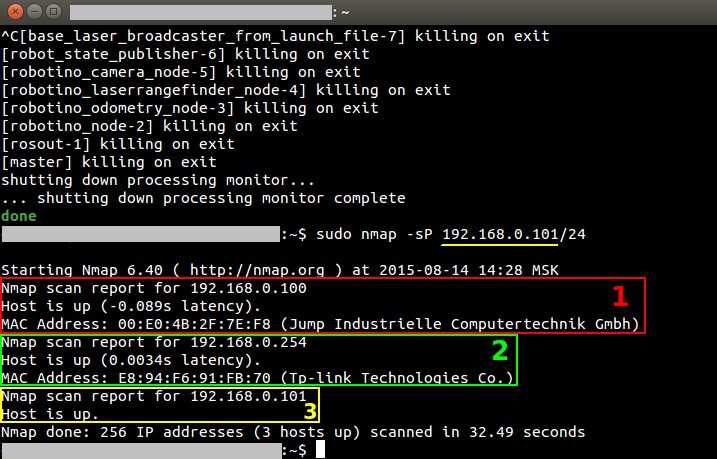
\includegraphics[width=\textwidth]{nmap.png}
	\caption{Работа утилиты nmap: 1~--- информация о компьютере Robotino, 2~--- о маршрутизаторе, 3~--- о компьютере, с которого проводилось сканирование.}
	\label{img_nmap}
\end{figure}

\begin{figure}[p]
	\centering
	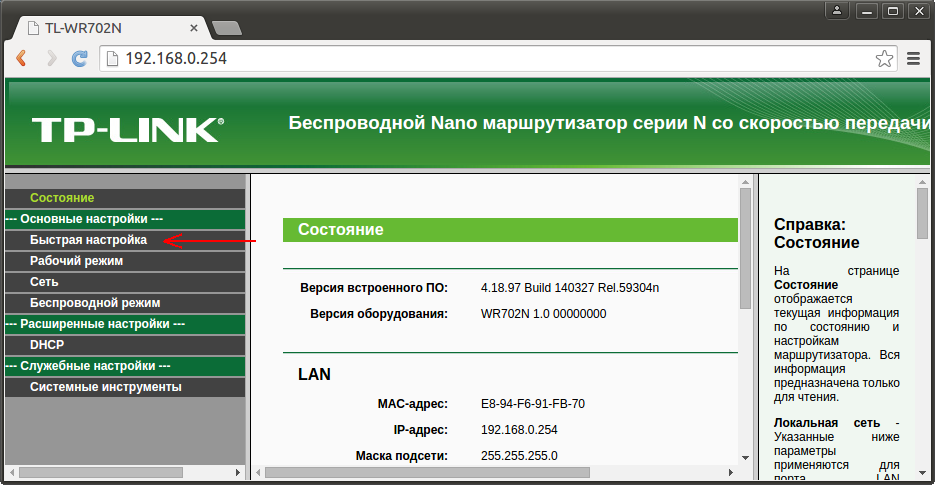
\includegraphics[width=\textwidth]{net_settings.png}
	\caption{Настройка роутера. Интерфейс.}
	\label{img_net_settings}
\end{figure}
